\documentclass[12pt,oneside]{article} % Uma Coluna e lingua portuguesa
%\usepackage[T1]{fontenc}        % Permite digitar os acentos de forma normal
\usepackage[utf8]{inputenc}
%\usepackage[english]{babel}
\usepackage[portuges,brazil]{babel}
%\usepackage[latin1]{inputenc}
\usepackage[dvips]{graphicx}    % Permite Gráficos
%\usepackage{times}    % Fonte Times
\usepackage{fancyhdr}
\usepackage{array}
\usepackage{multicol}
\usepackage[colorlinks=true,linkcolor=blue,urlcolor=blue]{hyperref}
\usepackage{nomencl}    % glossario
\usepackage{amssymb}
\usepackage{amsmath}
\usepackage[compact]{titlesec}
\usepackage{wrapfig}

%=======================================================================

% Hifenização das palavras desconhecidas pelo LaTeX
%\hyphenation{}
\paperheight    297mm
\paperwidth     210mm
\voffset         -15mm
\headheight      15pt %% tamanho de letra
\headsep         5mm  %% para o início do texto
\oddsidemargin  -3.0mm
\evensidemargin -3.0mm
\textwidth      167.0mm
\topmargin      005.0mm
\textheight     240.0mm
\footskip       10.0mm

\title{SAET 2022 - Maratona de Programação}

\author{Maratona de Programação}
\date{20 de Outubro de 2022}
\usepackage{indentfirst}
\usepackage{subfig}

\parindent=0pt
\setlength{\parskip}{7pt plus 1pt minus 2pt}
\titlespacing{\section}{0pt}{*0}{*0}
\titlespacing{\subsection}{0pt}{*0}{*0}
\titlespacing{\subsubsection}{0pt}{*0}{*0}

\begin{document}

\begin{center}
\textbf{\Huge SAET 2022 - Maratona de Programação} \\
\vspace{0.2cm}
\textit{20 de Outubro de 2022} \\
\vspace{1.0cm}
%\textbf{Sevidor BOCA:} \\
%\texttt{\large http://maratona.c3sl.ufpr.br/boca/} \\
%\vspace{1.0cm}
\begin{figure}[h!]
	\centering
 
\includegraphics[scale=0.95]{capa.png}
\end{figure}
\vspace{1.0cm}
%\textbf{Organizadores:}\\
%{\small Flávio Zavan} \\
%{\small Ricardo Oliveira} \\
\vspace{1.0cm}
\end{center}

\clearpage

\pagestyle{fancy}
\renewcommand{\footrulewidth}{0.7pt}
\renewcommand{\headrulewidth}{0.7pt}
\lhead{SAET 2022 - Maratona de Programação}
%\chead{Maratonas de Programação}
\rhead{20 de Outubro de 2022}
\cfoot{\thepage}

\newpage

% Espaco para o create-zips.sh nao achar
  \section*{Instruções Importantes}

\begin{itemize}

    \item Use a opção \textbf{Runs} para enviar suas soluções. Os problemas podem resolvidos em qualquer ordem e
    linguagem (dentre C, C++ e Python, independentemente do problema);

    \item Suas soluções serão testadas com várias entradas,
    além das dada como exemplo. Por isso, sua solução pode não ser
    aceita mesmo se funcionar para os exemplos dados. Certifique-se que ela
    funciona para todas as entradas possíveis;

    \item A saída gerada deve ser \textit{exatamente} conforme
    especificada. Em particular, \textbf{não} imprima instruções (``digite um
            número'', ``a resposta é'', etc);

    \item É garantido que todas as entradas usadas para teste estarão de acordo
    com o enunciado, não sendo necessário testar se são válidas;

    \item Ao enviar uma solução, o sistema irá responder uma das
    seguintes respostas:
    \begin{itemize}
        \item \verb|Not answered yet|: a solução está sendo corrigida.
        Aguarde um pouco e atualize a página;
        \item \verb|YES|: solução aceita. Parabéns!
        \item \verb|Wrong Answer|: a saída impressa pelo seu programa não é a
        saída correta esperada, para alguma entrada de teste;
        \item \verb|Presentation Error|: a saída impressa está correta, exceto
        por espaços em branco e/ou quebras-de-linha faltando/sobrando;
        \item \verb|Time Limit Exceeded|: o tempo de execução do seu programa
        ultrapassou o tempo limite estipulado para o problema (ver tabela
        abaixo). O tempo de execução da sua solução precisa ser menor;
        \item \verb|Runtime Error|: seu programa gerou algum erro em tempo de
        execução (``crashou'');
        \item \verb|Compile Error|: seu programa não compila.
    \end{itemize}

%    \item Sua solução será compilada com a seguinte linha de comando:
%    \begin{itemize}
%        \item C: \verb|gcc -static -O2 -lm|
%        \item C++: \verb|g++ -static -O2 -lm|
%        \item C++11: \verb|g++ -std=c++11 -static -O2 -lm|
%        \item Java: \verb|javac|
%        \item Pascal: \verb|fpc -Xt -XS -O2|
%    \end{itemize}

    \item Todas as linhas, tanto na entrada quanto na saída, terminam com o
    caractere de fim-de-linha ($\backslash n$), mesmo quando houver apenas uma única
    linha na entrada e/ou saída;

    \item Sua solução deve processar cada arquivo de entrada no tempo máximo
    estipulado para cada problema, dado pela seguinte tabela:

    \begin{table}[h]
    \centering
    \begin{tabular}{|c|c||c|}
    \hline
    \textbf{Problema} & \textbf{Nome} & \textbf{Tempo Limite (segundos)} \\
    \hline
    A & Funeral da Rainha & 1 \\
    \hline
    B & Herdeiros da Rainha & 1 \\
    \hline
    C & Rage Against the JVM & 4 \\
    \hline
    D & Quem não tem BIT caça com Seg & 1 \\
    \hline
    E & Logomarca & 1 \\
    \hline
    F & Resultado da Eleição & 1 \\
    \hline
    G & Álbum da Copa & 1 \\
    \hline
    H & Números Jares & 1 \\
    \hline
    I & Números Mares & 1 \\
    \hline
    J & Pesos na Barra & 1 \\
    \hline
    \end{tabular}
    \end{table}

 %   \item Os juizes usam um sistema de 64 bits (idêntico às maquinas do DINF).

%    \item Para submissões em \textbf{JAVA}, a classe deverá ter o mesmo nome que
%    o \textit{basename} do problema (leia a linha entre o título e o texto do
%    problema).

\end{itemize}

\newpage
\section*{A: Funeral da Rainha} %tle=1
\vspace{-0.52cm}
\noindent \begin{verbatim}Arquivo: funeral.[c|cpp|py]\end{verbatim}
A rainha morreu.

Por ela ter sido uma pessoa muito relevante para a história de seu país, o funeral
da rainha será aberto ao público e televisionado ao vivo para toda a nação.
Uma procissão aberta acontecerá durante o funeral, levando o caixão com o corpo
da monarca. A procissão sairá da Igreja Imperial (onde o corpo será velado) e
irá, em linha reta, até o Cemitério Real (onde o corpo será enterrado).

Preocupada com a segurança do evento, a organização da procissão decidiu que a
mesma não andará em velocidade constante durante todo o trajeto. Assim,
a organização demarcou $N$ pontos no trajeto, sendo o primeiro a $x_1$ metros da
Igreja; o segundo a $x_2$ metros da Igreja; etc., até o último ponto, a $x_N$
metros da Igreja, onde fica o Cemitério.

\begin{center}
    
\includegraphics[scale=0.8]{funeral/funeral.png}
\end{center}

Então, a
procissão sairá da Igreja, com velocidade inicial 0 (zero) e aceleração constante
$a_0$ m/s$^2$, até o ponto $x_1$. Neste ponto,
a aceleração é alterada para $a_1$ m/s$^2$, com a qual a procissão vai
até o ponto $x_2$. Neste ponto, a aceleração é alterada para $a_2$ m/s$^2$ e a
procissão segue até o ponto $x_3$; e assim por diante, até que a procissão chegue
ao Cemitério.

Para ajudar a organização com o restante do funeral, sua tarefa é determinar em
que horário a procissão chegará no Cemitério Real.


\subsection*{Entrada}

A primeira linha contém dois inteiros $N$ e $a_0$ ($1 \leq N \leq 10^4$, $0 <
        a_0 \leq 100$).
As próximas $N-1$ linhas contém, cada uma, os inteiros $x_i$ e $a_i$
($0 < x_i \leq 10^9$, $-100 \leq a_i \leq 100$).
A última linha contém o inteiro $x_N$ ($0 < x_N \leq 10^9$).

Os valores de $x_i$ são dados em ordem estritamente crescente, iniciando por $x_1$.
É garantido que a velocidade da procissão é sempre positiva durante todo o
trajeto (inclusive em todos os trechos em que a aceleração é negativa), e que é igual a zero apenas no ponto inicial (na Igreja).

\subsection*{Saída}

Imprima uma linha com um valor $T$, indicando que a procissão chegará no
Cemitério Real $T$ segundos após a saída da Igreja Imperial. Arredonde e imprima a resposta
com duas casas decimais.

\newpage
\begin{table}[!h]
\centering
\begin{tabular}{|l|l|}
\hline
\begin{minipage}[t]{3in}
\textbf{Exemplo de entrada}
\begin{verbatim}
1 3
100
\end{verbatim}
\vspace{1mm}
\end{minipage}
&
\begin{minipage}[t]{3in}
\textbf{Exemplo de saída}
\begin{verbatim}
8.16
\end{verbatim}
\vspace{1mm}
\end{minipage} \\
\hline
\end{tabular}
\end{table}

\begin{table}[!h]
\centering
\begin{tabular}{|l|l|}
\hline
\begin{minipage}[t]{3in}
\textbf{Exemplo de entrada}
\begin{verbatim}
2 3
50 5
100
\end{verbatim}
\vspace{1mm}
\end{minipage}
&
\begin{minipage}[t]{3in}
\textbf{Exemplo de saída}
\begin{verbatim}
7.97
\end{verbatim}
\vspace{1mm}
\end{minipage} \\
\hline
\end{tabular}
\end{table}

\begin{table}[!h]
\centering
\begin{tabular}{|l|l|}
\hline
\begin{minipage}[t]{3in}
\textbf{Exemplo de entrada}
\begin{verbatim}
5 10
60 5
120 -5
180 0
200 -6
295
\end{verbatim}
\vspace{1mm}
\end{minipage}
&
\begin{minipage}[t]{3in}
\textbf{Exemplo de saída}
\begin{verbatim}
11.64
\end{verbatim}
\vspace{1mm}
\end{minipage} \\
\hline
\end{tabular}
\end{table}


\newpage
\section*{B: Herdeiros da Rainha} %tle=1
\vspace{-0.52cm}
\noindent \begin{verbatim}Arquivo: herdeiros.[c|cpp|py]\end{verbatim}
A rainha morreu.

Imediatamente após o falecimento da monarca, o povo começou a
especular não apenas quem será o próximo rei, mas também quem
sentará no trono depois dele, e depois dele, e depois dele, etc. Em pouco tempo, saber toda a linha de sucessão ao
trono se tornou importantíssimo para a população.

Pelas regras da monarquia, o primeiro herdeiro ao trono é o filho mais
velho da rainha. Em seguida, vem os demais filhos da rainha, em ordem decrescente de
idade.

Após todos os filhos diretos da rainha, vem os filhos diretos do filho mais
velho dela. Em seguida, vem os filhos diretos do segundo filho mais velho da
rainha, e assim por diante.

Como exemplo, a figura abaixo apresenta uma possível árvore genealógica da família real,
indicando o ano de nascimento de cada herdeiro da rainha, e sua ordem na linha
de sucessão ao trono:

\begin{center}
    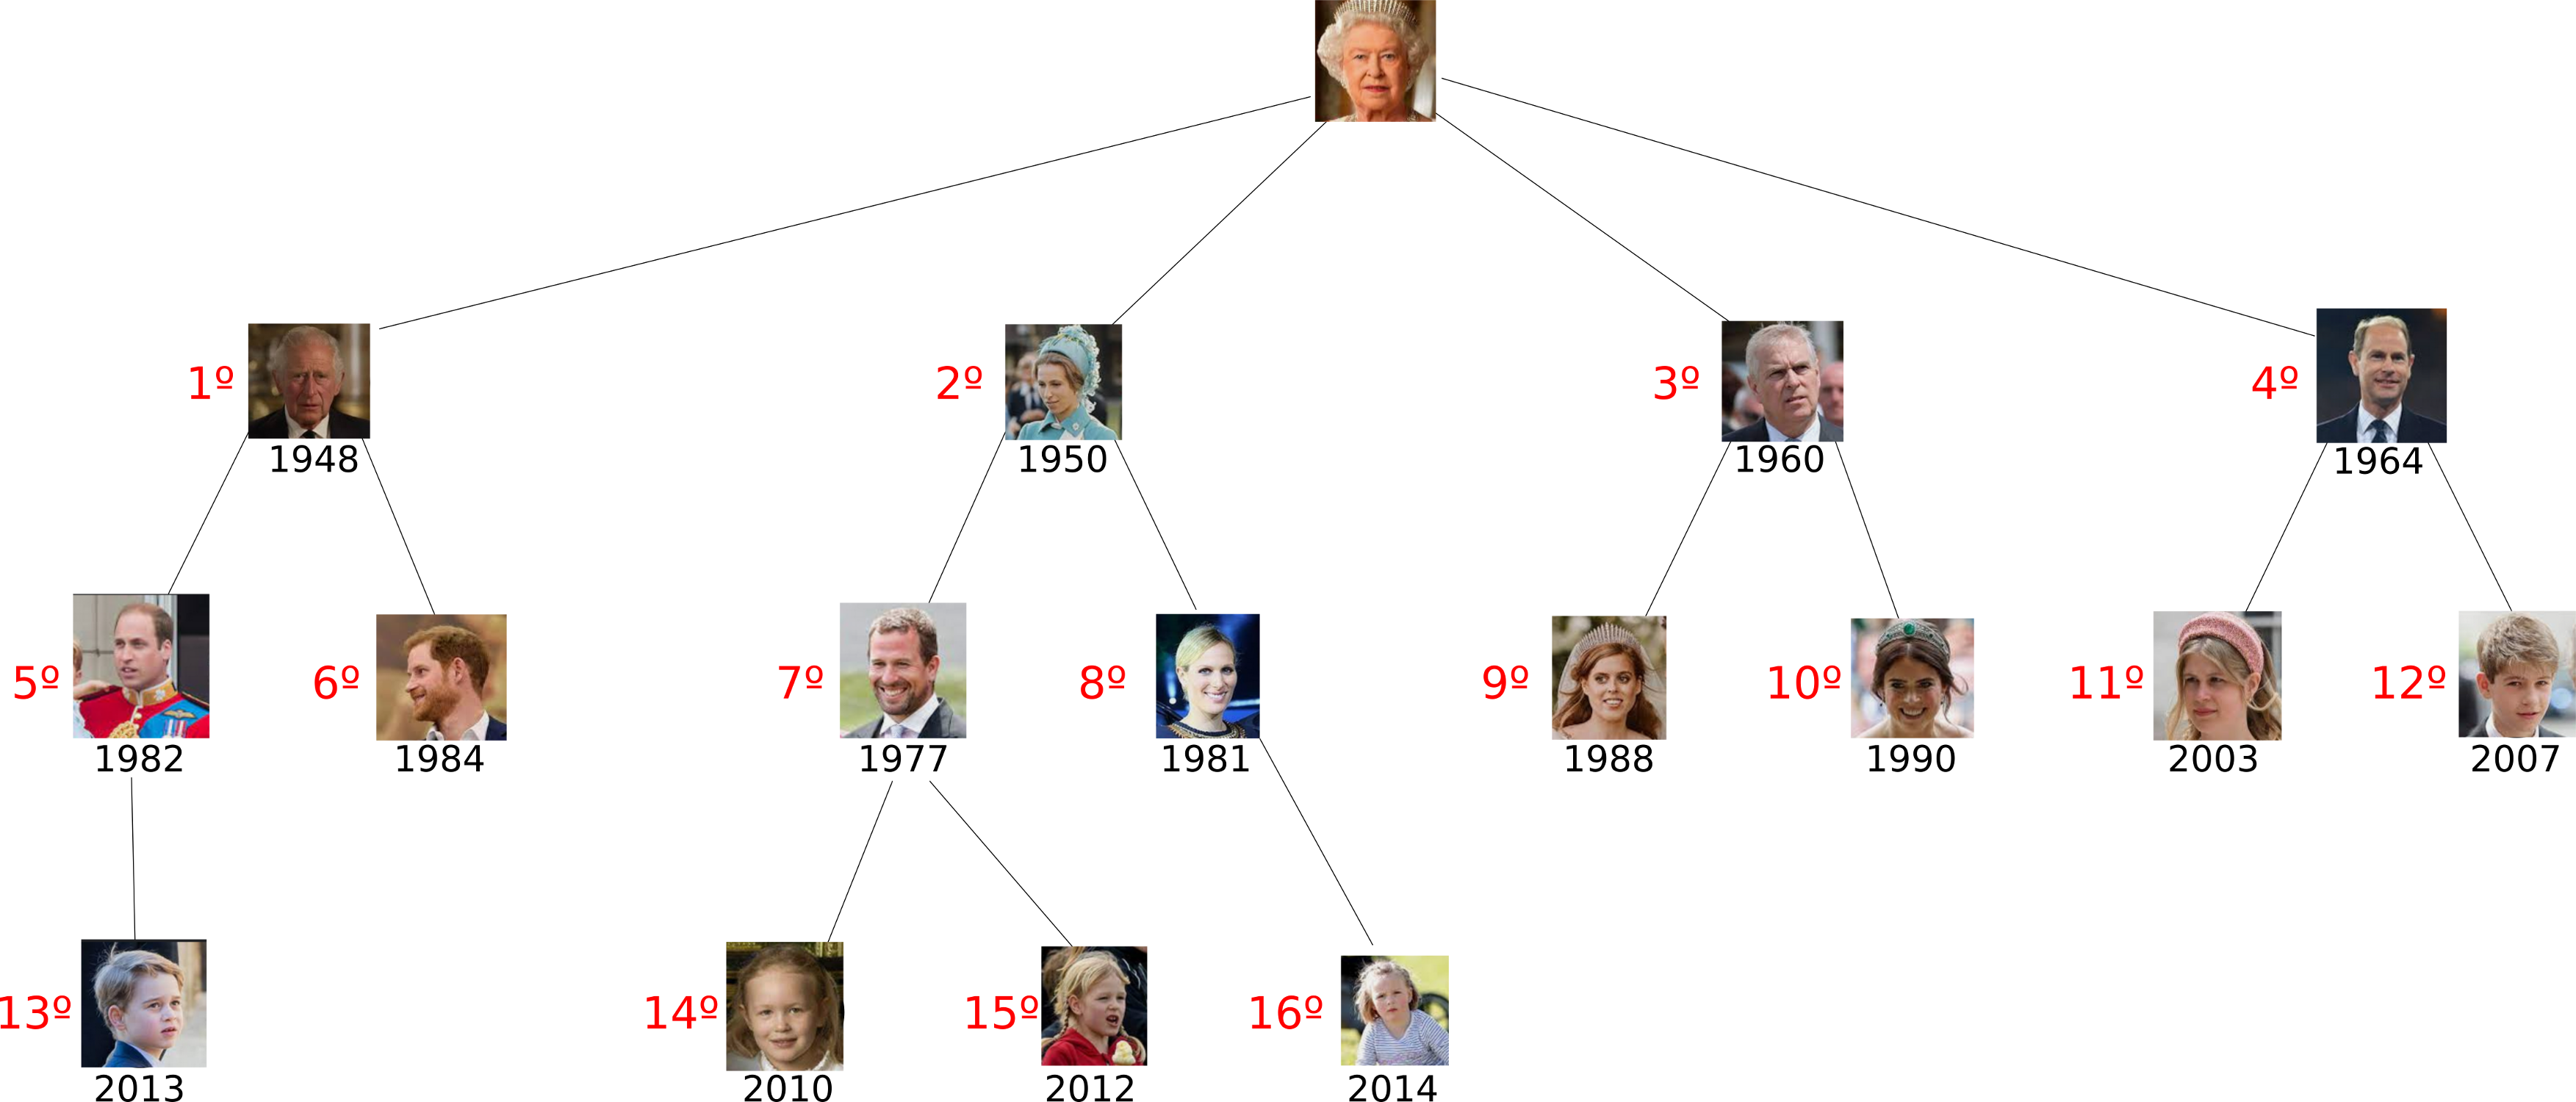
\includegraphics[scale=0.5]{herdeiros/herdeiros.png}
\end{center}

Dada a árvore genealógica da família real e o ano de nascimento de cada
herdeiro, determine toda a linha de sucessão ao trono.

\subsection*{Entrada}

A primeira linha contém um inteiro $N$ ($1 \leq N \leq 10^5$), o número de
herdeiros ao trono. Considere que os herdeiros são numerados de $1$ a $N$.
As próximas $N$ linhas descrevem um herdeiro cada. A linha $i$ $(1 \leq i \leq
        N)$ contém
dois inteiros $P_i$ e $D_i$ ($0 \leq P_i \leq N$, $0 \leq D_i \leq 10^5$), onde $P_i$ é o identificador do pai do herdeiro $i$ (ou 0 caso
o herdeiro $i$ seja filho direto da rainha), e $D_i$ é o ano de nascimento do
herdeiro $i$.

Não haverá dois herdeiros que nasceram no mesmo ano.

\subsection*{Saída}

Imprima $N$ linhas com os identificadores dos herdeiros, um por linha, na ordem
da linha de sucessão ao trono.

\newpage
\begin{table}[!h]
\centering
\begin{tabular}{|l|l|}
\hline
\begin{minipage}[t]{3in}
\textbf{Exemplo de entrada}
\begin{verbatim}
5
0 1961
0 1933
0 1957
0 2022
0 1970
\end{verbatim}
\vspace{1mm}
\end{minipage}
&
\begin{minipage}[t]{3in}
\textbf{Exemplo de saída}
\begin{verbatim}
2
3
1
5
4
\end{verbatim}
\vspace{1mm}
\end{minipage} \\
\hline
\end{tabular}
\end{table}



\begin{table}[!h]
\centering
\begin{tabular}{|l|l|}
\hline
\begin{minipage}[t]{3in}
\textbf{Exemplo de entrada}
\begin{verbatim}
16
2 1990
0 1960
5 1977
13 2014
0 1950
0 1964
9 1984
6 2007
0 1948
15 2013
3 2012
6 2003
5 1981
2 1988
9 1982
3 2010
\end{verbatim}
\vspace{1mm}
\end{minipage}
&
\begin{minipage}[t]{3in}
\textbf{Exemplo de saída}
\begin{verbatim}
9
5
2
6
15
7
3
13
14
1
12
8
10
16
11
4
\end{verbatim}
\vspace{1mm}
\end{minipage} \\
\hline
\end{tabular}
\end{table}


\newpage
\section*{C: Rage Against the JVM} %tle=4
\vspace{-0.52cm}
\noindent \begin{verbatim}Arquivo: rage.[c|cpp|py]\end{verbatim}
\vspace{-0.3cm}
Depois de uma viagem para lá de conturbada, finalmente as equipes
chegaram no local da Maratona de Programação deste ano. Ao
chegar, se depararam com um problema:
as máquinas, rodando nas problemáticas JVMs (\textit{Java Virtual Machine}),
estão travando demais.

Inicialmente, as equipes estão posicionadas em círculo, da equipe 1 à equipe
$N$, em sentido horário, e a equipe $i$ está utilizando a máquina $i$.
Quando acontece algum problema com as JVMs, a organização reinicia as máquinas e faz
um rodízio, no qual a máquina que cada equipe está usando
passa para a equipe que está a sua esquerda no círculo.

Cansadas, algumas equipes estão desistindo da competição e
indo embora. Quando uma equipe desiste, a máquina que ela estava utilizando é
descartada. Como exemplo, a figura abaixo apresenta: A) a posição inicial de
$N=4$ equipes e suas máquinas; B) o rodízio de máquinas após um problema; C) a
equipe 3 desistiu; D) o rodízio após outro problema.

\vspace{-0.4cm}
\begin{center}
    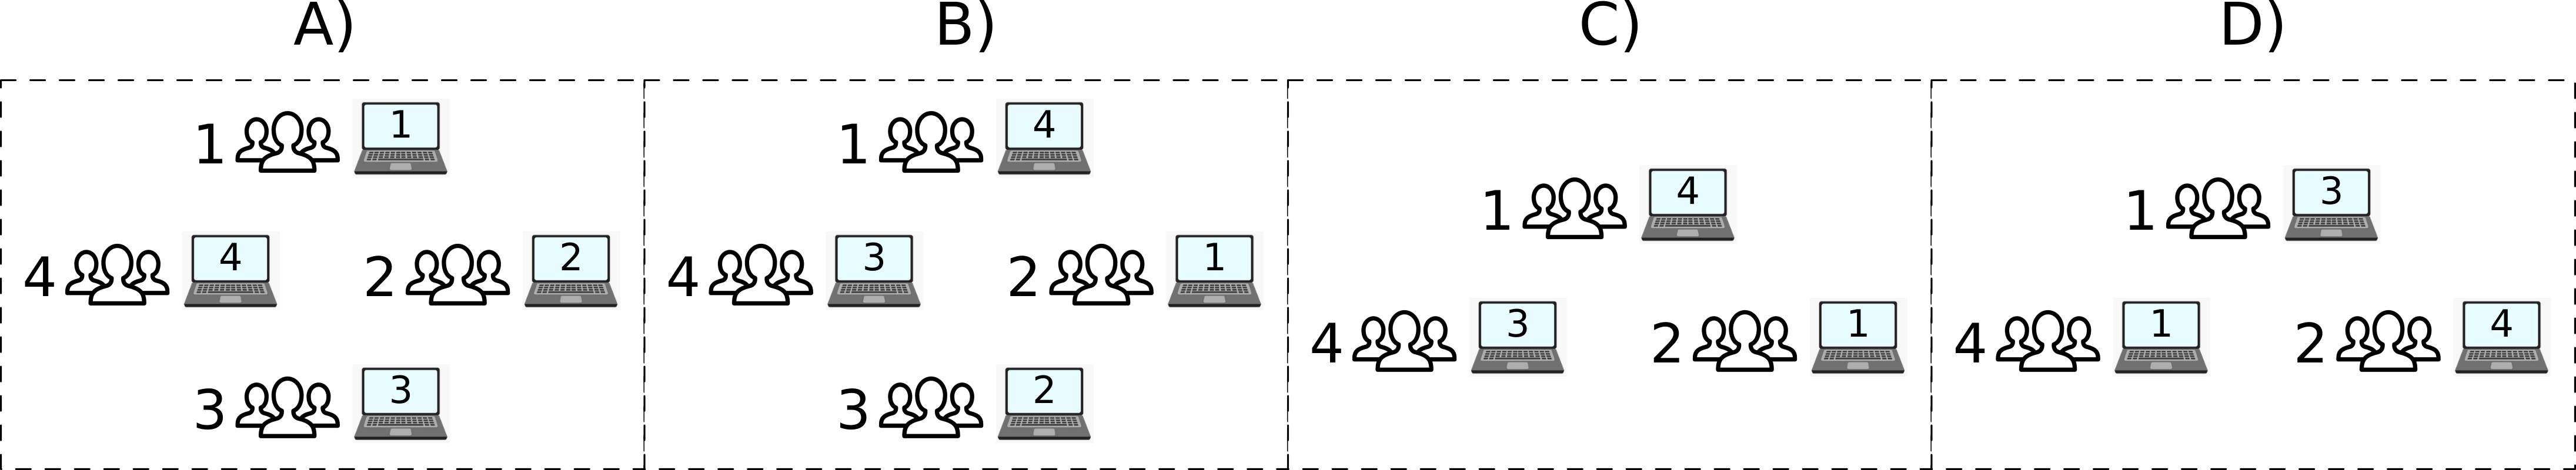
\includegraphics[scale=0.45]{rage/rage.png}
\end{center}

\vspace{-0.4cm}
Dada a sequência de problemas e de desistências que ocorreram, determine quais equipes
sobraram e com quais máquinas elas ficaram ao final da prova.

\subsection*{Entrada}

A primeira linha contém dois inteiros $N$ e $M$
($1 \leq N, M \leq 10^5$), o número de equipes e de acontecimentos,
respectivamente. A próxima linha contém $M$ inteiros $A_i$ indicando os
acontecimentos, na ordem em que aconteceram. $A_i=0$ indica um problema ocorrido
e um rodizio feito, enquanto $1 \leq A_i \leq N$ indica a desistência da equipe
$A_i$. Sobrará no mínimo uma equipe ao final da competição, e
nenhuma equipe desiste mais de uma vez.

\subsection*{Saída}

Para cada equipe que sobrou, imprima uma linha
com $i$ $c$ , indicando que a equipe $i$ ficou com a máquina $c$ no
final da prova.
Imprima em ordem crescente dos números das equipes.

\vspace{-0.3cm}
\begin{table}[!h]
\centering
\begin{tabular}{|l|l|}
\hline
\begin{minipage}[t]{3in}
\textbf{Exemplo de entrada}
\begin{verbatim}
4 3
0 3 0
\end{verbatim}
\vspace{1mm}
\end{minipage}
&
\begin{minipage}[t]{3in}
\textbf{Exemplo de saída}
\begin{verbatim}
1 3
2 4
4 1
\end{verbatim}
\vspace{1mm}
\end{minipage} \\
\hline
\end{tabular}
\end{table}

\vspace{-0.3cm}
\begin{table}[!h]
\centering
\begin{tabular}{|l|l|}
\hline
\begin{minipage}[t]{3in}
\textbf{Exemplo de entrada}
\begin{verbatim}
3 3
0 0 1
\end{verbatim}
\vspace{1mm}
\end{minipage}
&
\begin{minipage}[t]{3in}
\textbf{Exemplo de saída}
\begin{verbatim}
2 3
3 1
\end{verbatim}
\vspace{1mm}
\end{minipage} \\
\hline
\end{tabular}
\end{table}


\newpage
\section*{D: Quem não tem BIT caça com Seg} %tle=1
\vspace{-0.52cm}
\noindent \begin{verbatim}Arquivo: bit.[c|cpp|py]\end{verbatim}
Enquanto preparava suas anotações para levar para a Maratona de Programação,
Douglas percebeu um fato interessante: algumas estruturas de dados fazem tudo o
que outras estruturas fazem e mais um pouco, e logo poderiam substitui-las sem
prejuizo. É o caso, por exemplo, da BIT (\textit{Binary Indexed Tree}) e da Seg
(\textit{Segment Tree}). A Seg tem todas as funcionalidades que a BIT tem (além
        das funcionalidades que só a Seg possui). Por isso, conhecer a
BIT não é \textit{realmente} necessário quando se já conhece a Seg\footnote{embora é recomendado, pois o
código da BIT é mais compacto que o da Seg, tornando-a mais prática.}, pois todo problema que pode
ser resolvido com a BIT pode ser resolvido com a Seg em seu lugar. Neste caso,
    dizemos que a Seg \textit{pode substituir} a BIT.

Após estudar todas as $N$ estruturas de dados que existem, Douglas descobriu quais
estruturas podem substituir quais outras. Agora Douglas está curioso: qual é a estrutura
de dados que pode substituir (direta ou indiretamente) a maior quantidade de outras estruturas?

\subsection*{Entrada}

A primeira linha contém dois inteiros $N$ e $M$
($1 \leq N \leq 2000, 0 \leq M \leq min(\frac{N^2 - N}{2}, 2000$)), o número de estruturas e de substituições,
respectivamente. As estruturas são numeradas de $1$ a $N$.
As próximas $M$ linhas contém dois inteiros $A$ e $B$ cada
$(1 \leq A, B \leq N, A \neq B)$, indicando que a estrutura $A$ pode substituir a
estrutura $B$.

É garantido que a relação de substituições não contém ciclos.

\subsection*{Saída}

Imprima uma linha com dois inteiros $E$ e $S$, onde $E$ é a estrutura de dados
que pode substituir (direta ou indiretamente) a maior quantidade de outras estruturas, enquanto $S$ é a quantidade
de outras estruturas que $E$ pode substituir (direta ou indiretamente).

Se houver mais de uma estrutura que pode substituir a maior quantidade de estruturas,
imprima a de menor número identificador.

\vspace{-0.3cm}
\begin{table}[!h]
\centering
\begin{tabular}{|l|l|}
\hline
\begin{minipage}[t]{3in}
\textbf{Exemplo de entrada}
\begin{verbatim}
8 9
1 2
2 5
2 6
5 6
3 2
7 6
3 7
4 3
8 7
\end{verbatim}
\vspace{1mm}
\end{minipage}
&
\begin{minipage}[t]{3in}
\textbf{Exemplo de saída}
\begin{verbatim}
4 5
\end{verbatim}
\vspace{1mm}
\end{minipage} \\
\hline
\end{tabular}
\end{table}


\newpage
\section*{E: Logomarca} %tle=1
\vspace{-0.52cm}
\noindent \begin{verbatim}Arquivo: logomarca.[c|cpp|py]\end{verbatim}
\vspace{-0.4cm}
Rodriguinho está muito animado com a empresa de serviços em TI que está abrindo.
Após já ter decidido o nome da empresa e o endereço onde o escritório será
instalado, Rodriguinho está agora definindo uma logomarca para a empresa.

Minimalista que é, ele decidiu que a logo consistirá apenas de um círculo
cortado por duas retas verticais, com a área entre elas pintadas de alguma cor
(a cor vai mudar a cada mês).

Para simplificar, considere que o círculo tem centro na origem do plano
cartesiano e tem raio $r$, e que as retas verticais cortam o eixo X nos
pontos $x_1$ e $x_2$. Como exemplo, a figura abaixo apresenta
uma logo com $r=5, x_1=-2, x_2=1$:

\vspace{-0.5cm}
\begin{center}
    %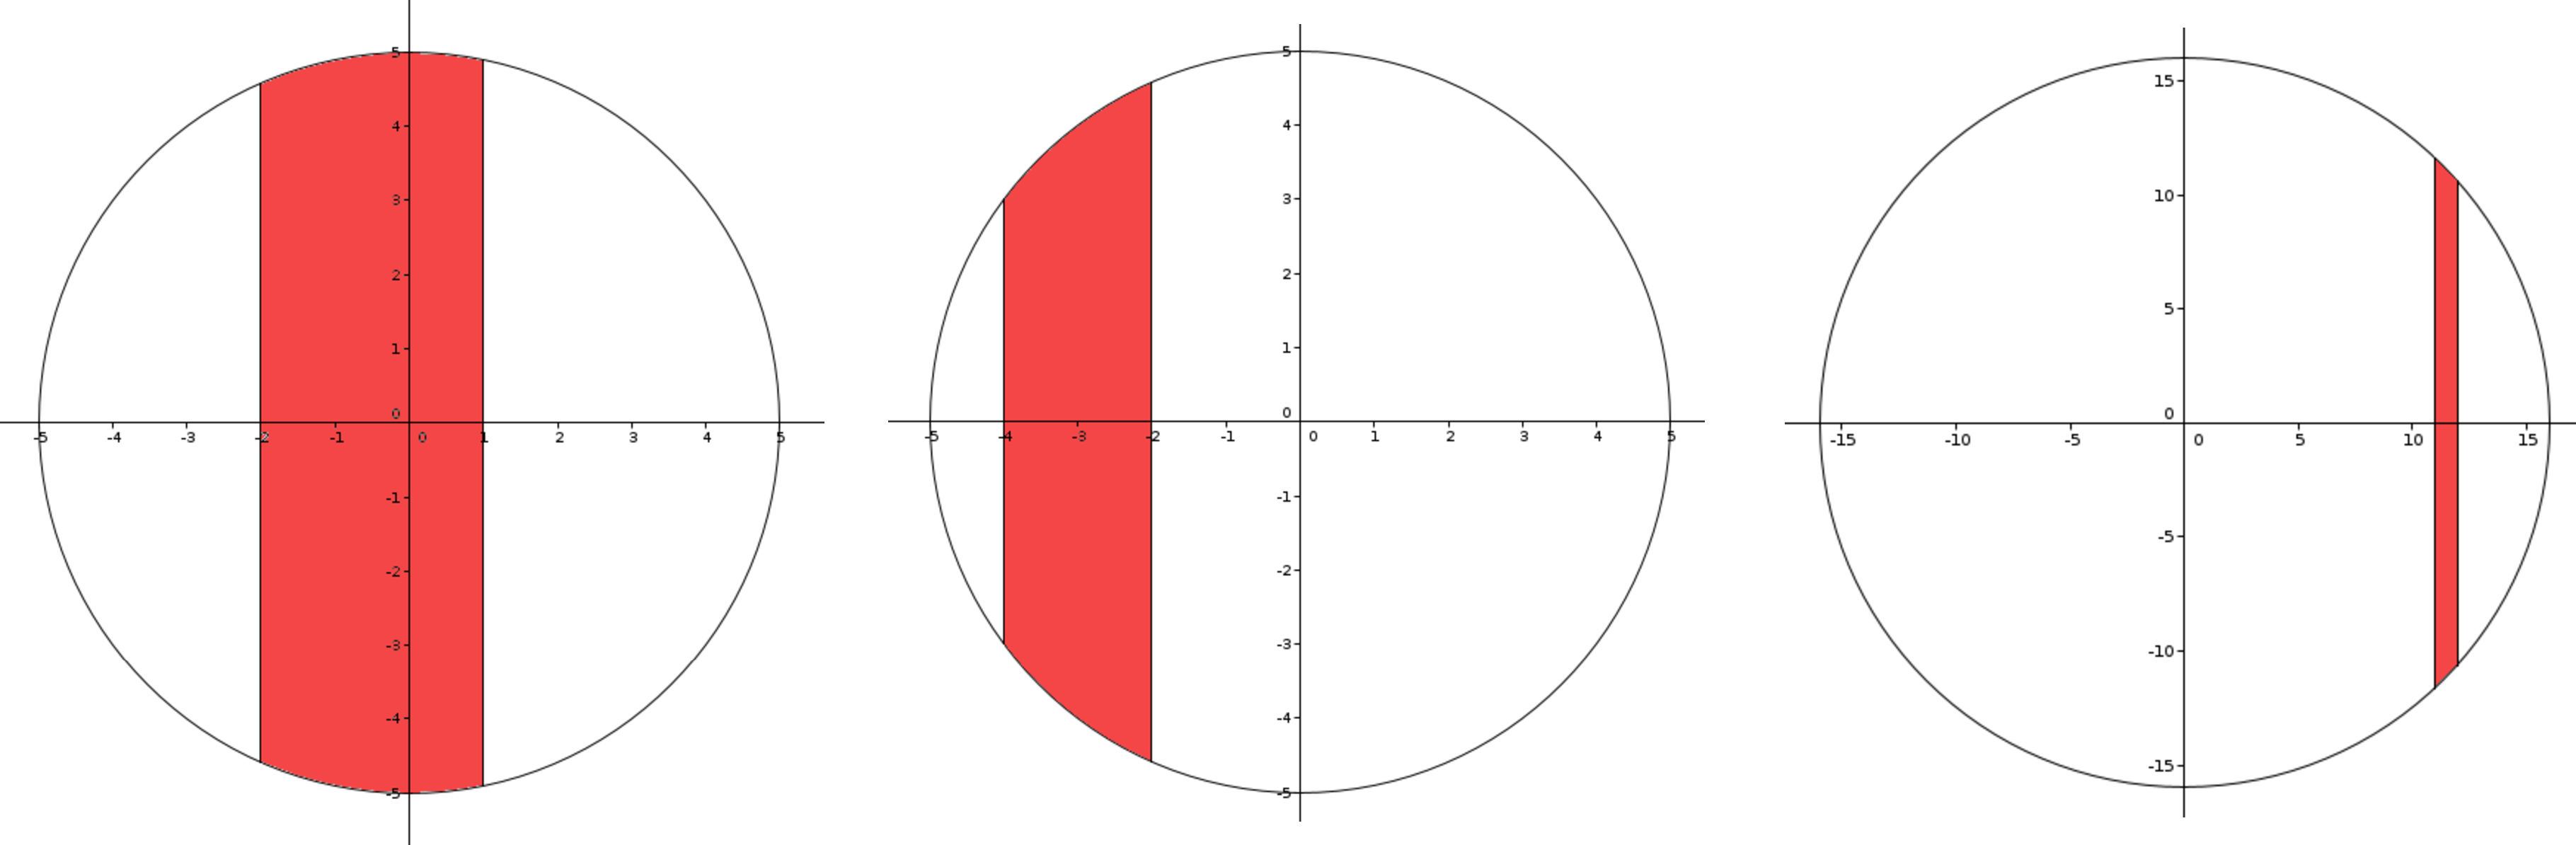
\includegraphics[scale=0.2]{logomarca/logomarca.pdf}
    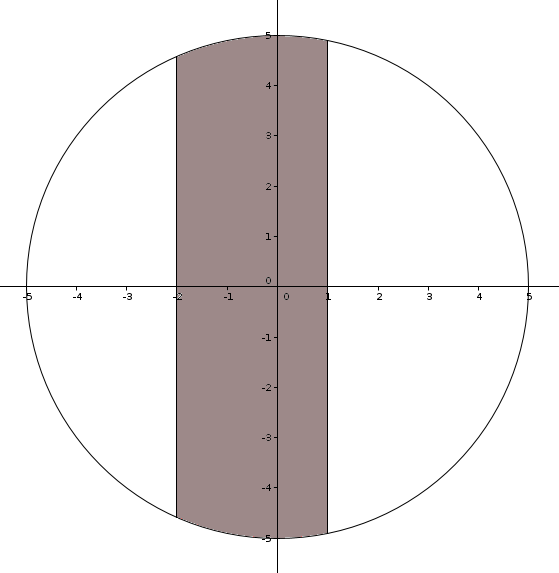
\includegraphics[scale=0.3]{logomarca/logo1.png}
\end{center}

\vspace{-0.5cm}
Rodriguinho está preocupado com a quantidade de tinta que terá de comprar todos
os meses. Por isso, ele pediu sua ajuda para
determinar a área da região pintada na sua logomarca.


\subsection*{Entrada}

A única linha da entrada contém três inteiros $r$, $x_1$ e $x_2$
($1 \leq r \leq 50$, $-r \leq x_1 < x_2 \leq r$).

\subsection*{Saída}

Imprima uma linha contendo a área da região pintada, arredondada com três casas decimais.

\begin{table}[!h]
\centering
\begin{tabular}{|l|l|}
\hline
\begin{minipage}[t]{3in}
\textbf{Exemplo de entrada}
\begin{verbatim}
5 -2 1
\end{verbatim}
\vspace{1mm}
\end{minipage}
&
\begin{minipage}[t]{3in}
\textbf{Exemplo de saída}
\begin{verbatim}
29.386
\end{verbatim}
\vspace{1mm}
\end{minipage} \\
\hline
\end{tabular}
\end{table}

\begin{table}[!h]
\centering
\begin{tabular}{|l|l|}
\hline
\begin{minipage}[t]{3in}
\textbf{Exemplo de entrada}
\begin{verbatim}
5 -4 -2
\end{verbatim}
\vspace{1mm}
\end{minipage}
&
\begin{minipage}[t]{3in}
\textbf{Exemplo de saída}
\begin{verbatim}
15.729
\end{verbatim}
\vspace{1mm}
\end{minipage} \\
\hline
\end{tabular}
\end{table}

\begin{table}[!h]
\centering
\begin{tabular}{|l|l|}
\hline
\begin{minipage}[t]{3in}
\textbf{Exemplo de entrada}
\begin{verbatim}
16 11 12
\end{verbatim}
\vspace{1mm}
\end{minipage}
&
\begin{minipage}[t]{3in}
\textbf{Exemplo de saída}
\begin{verbatim}
22.233
\end{verbatim}
\vspace{1mm}
\end{minipage} \\
\hline
\end{tabular}
\end{table}


\newpage
\section*{F: Resultado da Eleição} %tle=1
\vspace{-0.52cm}
\noindent \begin{verbatim}Arquivo: resultado.[c|cpp|py]\end{verbatim}
Este ano temos eleições gerais para escolher o novo chefe de governo da Nlogonia.

Cada um dos $N$ eleitores do país tem três opções de como
votar no dia da eleição: votar em um dos $M$
candidatos que estão concorrendo ao cargo; votar em branco; ou anular seu
voto.

Um \textit{voto válido} é um voto dado em algum dos $M$ candidatos (isto é, um voto
que não é nem em branco nem nulo). Se algum candidato receber mais que $50\%$
de todos os votos válidos, ele vence a eleição. Caso contrário,
os dois candidatos que mais receberem votos válidos irão disputar uma nova
eleição, em segundo turno.

Chegou a hora de totalizar os votos! Dados os votos registrados nas urnas, algum
candidato venceu a eleição? Ou haverá segundo turno?

\subsection*{Entrada}

A primeira linha contém dois inteiros $N$ e $M$
($1 \leq N, M \leq 10^5$), o número de eleitores e de candidatos,
respectivamente. Os candidatos são numerados de $1$ a $M$.
A próxima linha contém $N$ votos. Cada voto pode ser um número de um cadidato, a
letra \verb|B| (voto em branco) ou a letra \verb|N| (voto nulo).

É garantido que a entrada contém no mínimo 1 voto válido, e que, se houver
segundo turno, não haverá empate nem na primeira nem na segunda colocação.

\subsection*{Saída}

Se não houver segundo turno, imprima uma linha contendo
\verb|vencedor |$C$, sendo $C$ o número do candidato vencedor. Caso contrário,
    imprima uma linha contendo \verb|segundo turno entre |$A$\verb| e |$B$, onde
    $A$ e $B$ são os números do candidato mais votado e o segundo mais votado,
    respectivamente.


\begin{table}[!h]
\centering
\begin{tabular}{|l|l|}
\hline
\begin{minipage}[t]{3in}
\textbf{Exemplo de entrada}
\begin{verbatim}
7 100
92 92 B 7 92 7 N
\end{verbatim}
\vspace{1mm}
\end{minipage}
&
\begin{minipage}[t]{3in}
\textbf{Exemplo de saída}
\begin{verbatim}
vencedor 92
\end{verbatim}
\vspace{1mm}
\end{minipage} \\
\hline
\end{tabular}
\end{table}

\begin{table}[!h]
\centering
\begin{tabular}{|l|l|}
\hline
\begin{minipage}[t]{3in}
\textbf{Exemplo de entrada}
\begin{verbatim}
11 100
B 95 N 95 95 99 99 B 95 98 99
\end{verbatim}
\vspace{1mm}
\end{minipage}
&
\begin{minipage}[t]{3in}
\textbf{Exemplo de saída}
\begin{verbatim}
segundo turno entre 95 e 99
\end{verbatim}
\vspace{1mm}
\end{minipage} \\
\hline
\end{tabular}
\end{table}

\begin{table}[!h]
\centering
\begin{tabular}{|l|l|}
\hline
\begin{minipage}[t]{3in}
\textbf{Exemplo de entrada}
\begin{verbatim}
10 10
9 B 5 N 5 9 B 5 9 5
\end{verbatim}
\vspace{1mm}
\end{minipage}
&
\begin{minipage}[t]{3in}
\textbf{Exemplo de saída}
\begin{verbatim}
vencedor 5
\end{verbatim}
\vspace{1mm}
\end{minipage} \\
\hline
\end{tabular}
\end{table}


\newpage
\section*{G: Álbum da Copa} %tle=1
\vspace{-0.52cm}
\noindent \begin{verbatim}Arquivo: album.[c|cpp|py]\end{verbatim}
No mês que vem começa a grande Copa do Mundo de Dados Estruturados de 2022, que
este ano acontece na grande cidade de Touledow. Para motivar as pessoas a
acompanherem o torneio\footnote{o que os jovens de hoje chamam de ``hypar'' o
evento}, diversas ações de publicidade e \textit{merchandising}
estão sendo feitas durante o ano todo.

Em uma dessas ações, a organização lançou o Álbum de Figurinhas Oficial da
Copa$^\circledR$. O álbum é composto por $N$ figurinhas distintas, numeradas de
1 a $N$. Para completar o álbum, é necessário obter pelo menos uma cópia de cada
uma dessas $N$ figurinhas.

Ana tem uma coleção de figurinhas que pode não conter todas as figurinhas de 1
a $N$, e pode conter algumas figurinhas repetidas. Beto também tem uma coleção
de figurinhas com as mesmas condições.

Para poderem completar seus álbuns, Ana e Beto irão trocar figurinhas.
Em uma troca, Ana dá uma figurinha para Beto e, ao mesmo tempo,
Beto dá uma figurinha para Ana. Note que apenas \textit{trocas} são
permitidas -- uma pessoa não irá dar uma figurinha para outra sem receber uma
outra figurinha em troca.

Determine o menor número de trocas necessário para que ambos completem seus
álbuns, ou indique que isso não é possível.

\subsection*{Entrada}

A primeira linha contém o inteiro $N$ ($1 \leq N \leq 1000$).

A próxima linha
contém $N_A$ ($1 \leq N_A \leq 1000$), o número de figurinhas de Ana.

A próxima
linha contém $N_A$ inteiros de 1 a $N$, indicando quais figurinhas Ana tem.

A próxima linha
contém $N_B$ ($1 \leq N_B \leq 1000$), o número de figurinhas de Beto.

A próxima
linha contém $N_B$ inteiros de 1 a $N$, indicando quais figurinhas Beto tem.

\subsection*{Saída}

Imprima uma única linha contendo o número mínimo de trocas necessárias, ou
\verb|impossivel| se não for possível que ambos completem seus álbuns trocando
figurinhas.

\newpage
\begin{table}[!h]
\centering
\begin{tabular}{|l|l|}
\hline
\begin{minipage}[t]{3in}
\textbf{Exemplo de entrada}
\begin{verbatim}
5
5
1 1 2 4 5
5
2 3 3 4 5
\end{verbatim}
\vspace{1mm}
\end{minipage}
&
\begin{minipage}[t]{3in}
\textbf{Exemplo de saída}
\begin{verbatim}
1
\end{verbatim}
\vspace{1mm}
\end{minipage} \\
\hline
\end{tabular}
\end{table}

\begin{table}[!h]
\centering
\begin{tabular}{|l|l|}
\hline
\begin{minipage}[t]{3in}
\textbf{Exemplo de entrada}
\begin{verbatim}
5
6
1 1 2 4 5 5
5
2 3 3 3 4
\end{verbatim}
\vspace{1mm}
\end{minipage}
&
\begin{minipage}[t]{3in}
\textbf{Exemplo de saída}
\begin{verbatim}
2
\end{verbatim}
\vspace{1mm}
\end{minipage} \\
\hline
\end{tabular}
\end{table}

\begin{table}[!h]
\centering
\begin{tabular}{|l|l|}
\hline
\begin{minipage}[t]{3in}
\textbf{Exemplo de entrada}
\begin{verbatim}
5
6
1 1 2 4 5 5
4
2 3 3 4
\end{verbatim}
\vspace{1mm}
\end{minipage}
&
\begin{minipage}[t]{3in}
\textbf{Exemplo de saída}
\begin{verbatim}
impossivel
\end{verbatim}
\vspace{1mm}
\end{minipage} \\
\hline
\end{tabular}
\end{table}

\begin{table}[!h]
\centering
\begin{tabular}{|l|l|}
\hline
\begin{minipage}[t]{3in}
\textbf{Exemplo de entrada}
\begin{verbatim}
10
13
9 1 7 1 3 3 5 3 5 9 7 7 9
12
6 2 4 2 10 4 8 4 6 8 6 10
\end{verbatim}
\vspace{1mm}
\end{minipage}
&
\begin{minipage}[t]{3in}
\textbf{Exemplo de saída}
\begin{verbatim}
5
\end{verbatim}
\vspace{1mm}
\end{minipage} \\
\hline
\end{tabular}
\end{table}


\newpage
\section*{H: Números Jares} %tle=1
\vspace{-0.52cm}
\noindent \begin{verbatim}Arquivo: jares.[c|cpp|py]\end{verbatim}
\vspace{-0.5cm}
Sempre que o prof. Racirdinho fala sobre números pares e números ímpares durante
as aulas de Teoria da Poncutação, uma dúvida geral surge: ``o número 0 (zero) é
par?''.

Embora o professor insista que zero seja sim um número par, Joãozinho ainda está
desconfiado desta informação, e prefere não tomar isso como verdade. Para não
gerar conflitos, Joãozinho decidiu criar sua própria definição de números pares.

Um número é \textit{jar} (abreviação para ``Joãozinho-par'') se é positivo, é
múltiplo de dois, e não termina com zero em sua representação decimal.
Desta forma, os primeiros números jares são 2, 4, 6, 8, 12, 14, 16, 18, 22, ....
Dado um número inteiro, determine se ele é um número jar.

\subsection*{Entrada}

A única linha da entrada contém um inteiro $N$ ($-10^9 \leq N \leq 10^9$).

\subsection*{Saída}

Imprima uma única linha contendo \verb|sim| se $N$ é um número jar, ou
\verb|nao| caso contrário.

\begin{table}[!h]
\centering
\begin{tabular}{|l|l|}
\hline
\begin{minipage}[t]{3in}
\textbf{Exemplo de entrada}
\begin{verbatim}
0
\end{verbatim}
\vspace{1mm}
\end{minipage}
&
\begin{minipage}[t]{3in}
\textbf{Exemplo de saída}
\begin{verbatim}
nao
\end{verbatim}
\vspace{1mm}
\end{minipage} \\
\hline
\end{tabular}
\end{table}

\begin{table}[!h]
\centering
\begin{tabular}{|l|l|}
\hline
\begin{minipage}[t]{3in}
\textbf{Exemplo de entrada}
\begin{verbatim}
42
\end{verbatim}
\vspace{1mm}
\end{minipage}
&
\begin{minipage}[t]{3in}
\textbf{Exemplo de saída}
\begin{verbatim}
sim
\end{verbatim}
\vspace{1mm}
\end{minipage} \\
\hline
\end{tabular}
\end{table}

\begin{table}[!h]
\centering
\begin{tabular}{|l|l|}
\hline
\begin{minipage}[t]{3in}
\textbf{Exemplo de entrada}
\begin{verbatim}
100
\end{verbatim}
\vspace{1mm}
\end{minipage}
&
\begin{minipage}[t]{3in}
\textbf{Exemplo de saída}
\begin{verbatim}
nao
\end{verbatim}
\vspace{1mm}
\end{minipage} \\
\hline
\end{tabular}
\end{table}

\begin{table}[!h]
\centering
\begin{tabular}{|l|l|}
\hline
\begin{minipage}[t]{3in}
\textbf{Exemplo de entrada}
\begin{verbatim}
102
\end{verbatim}
\vspace{1mm}
\end{minipage}
&
\begin{minipage}[t]{3in}
\textbf{Exemplo de saída}
\begin{verbatim}
sim
\end{verbatim}
\vspace{1mm}
\end{minipage} \\
\hline
\end{tabular}
\end{table}

\begin{table}[!h]
\centering
\begin{tabular}{|l|l|}
\hline
\begin{minipage}[t]{3in}
\textbf{Exemplo de entrada}
\begin{verbatim}
642487
\end{verbatim}
\vspace{1mm}
\end{minipage}
&
\begin{minipage}[t]{3in}
\textbf{Exemplo de saída}
\begin{verbatim}
nao
\end{verbatim}
\vspace{1mm}
\end{minipage} \\
\hline
\end{tabular}
\end{table}

\begin{table}[!h]
\centering
\begin{tabular}{|l|l|}
\hline
\begin{minipage}[t]{3in}
\textbf{Exemplo de entrada}
\begin{verbatim}
-2
\end{verbatim}
\vspace{1mm}
\end{minipage}
&
\begin{minipage}[t]{3in}
\textbf{Exemplo de saída}
\begin{verbatim}
nao
\end{verbatim}
\vspace{1mm}
\end{minipage} \\
\hline
\end{tabular}
\end{table}


\newpage
\section*{I: Números Mares} %tle=1
\vspace{-0.52cm}
\noindent \begin{verbatim}Arquivo: mares.[c|cpp|py]\end{verbatim}
\vspace{-0.5cm}
Sempre que o prof. Racirdinho fala sobre números pares e números ímpares durante
as aulas de Teoria da Poncutação, uma dúvida geral surge: ``o número 0 (zero) é
par?''.

Embora o professor insista que zero seja sim um número par, Mariazinha ainda está
desconfiada desta informação, e prefere não tomar isso como verdade. Para não
gerar conflitos, Mariazinha decidiu criar sua própria definição de números pares.

Um número é \textit{mar} (abreviação para ``Mariazinha-par'') se é positivo, é
múltiplo de dois, e não contém nenhum 0 (zero) em sua representação decimal.
Como exemplo, os números 2, 42, e 796 são mares, enquanto 0, 20, 402 e 7096 não são
mares.

Os primeiros números mares são, nesta ordem, 2, 4, 6, 8, 12, 14, 16, 18, 22, 24, etc.
Sua tarefa é, para várias consultas, determinar, dado um inteiro $N$, qual é o $N-$ésimo número mar.

\subsection*{Entrada}

A primeira linha contém um inteiro $Q$ ($1 \leq Q \leq 100$), o número de
consultas. As próximas $Q$ linhas descrevem uma consulta cada.
Cada linha contém um inteiro $N$ ($1 \leq N \leq 10^{15}$).

\subsection*{Saída}

Para cada consulta, imprima uma linha contendo o $N-$ésimo número mar.

\begin{table}[!h]
\centering
\begin{tabular}{|l|l|}
\hline
\begin{minipage}[t]{3in}
\textbf{Exemplo de entrada}
\begin{verbatim}
6
1
2
10
100
38
1000
\end{verbatim}
\vspace{1mm}
\end{minipage}
&
\begin{minipage}[t]{3in}
\textbf{Exemplo de saída}
\begin{verbatim}
2
4
24
268
94
2968
\end{verbatim}
\vspace{1mm}
\end{minipage} \\
\hline
\end{tabular}
\end{table}


\newpage
\section*{J: Pesos na Barra} %tle=1
\vspace{-0.52cm}
\noindent \begin{verbatim}Arquivo: pesos.[c|cpp|py]\end{verbatim}
\vspace{-0.4cm}
\textit{``Em pleno 2022; ano da tecnologia; ano da
eleição; ano da copa; ano em que empresários bilionários estão construindo
    foguetes; neste ano, é
necessário malhar bastante na academia''}. Com essa filosofia em mente, Gustavo vai
à academia treinar todos os dias depois do trabalho.

Diversos exercícios da academia envolvem encaixar anilhas (pesos em forma de
disco) nas duas pontas de uma barra de ferro, para então erguer a barra em uma
posição que favorece determinado músculo.
Para que o exercício seja executado corretamente, é necessário que o peso total
em uma ponta da barra seja igual ao peso total na outra ponta da barra, como no
exemplo abaixo:

\vspace{-0.4cm}
\begin{center}
    
\includegraphics[scale=0.5]{pesos/pesos.png}
\end{center}

\vspace{-0.5cm}
Gustavo quer treinar o máximo possível e, por isso, quer usar
\textit{todas} as anilhas disponíveis na academia.
Dadas as anilhas disponíveis e seus pesos, é possível distribuir \textit{todas}
as anilhas nas duas pontas da barra de forma que o peso total seja o mesmo em ambas?

\subsection*{Entrada}

A primeira linha contém o inteiro $N$ ($1 \leq N \leq 100$), o número de
anilhas disponíveis. A segunda linha contém $N$ inteiros $P_i$ ($1 \leq P_i \leq 100$), o
peso de cada anilha, em quilogramas.

Considere que a barra é comprida o bastante de forma que é possível colocar
qualquer quantidade de anilhas, em ambas as pontas.

\subsection*{Saída}

Imprima uma única linha contendo \verb|SIM| se é possível distribuir todas as
anilhas nas duas pontas da barra de forma que o peso total seja o mesmo em
ambas, ou \verb|NAO| caso contrário.

\begin{table}[!h]
\centering
\begin{tabular}{|l|l|}
\hline
\begin{minipage}[t]{3in}
\textbf{Exemplo de entrada}
\begin{verbatim}
4
5 20 5 10
\end{verbatim}
\vspace{1mm}
\end{minipage}
&
\begin{minipage}[t]{3in}
\textbf{Exemplo de saída}
\begin{verbatim}
SIM
\end{verbatim}
\vspace{1mm}
\end{minipage} \\
\hline
\end{tabular}
\end{table}

\begin{table}[!h]
\centering
\begin{tabular}{|l|l|}
\hline
\begin{minipage}[t]{3in}
\textbf{Exemplo de entrada}
\begin{verbatim}
3
20 5 10
\end{verbatim}
\vspace{1mm}
\end{minipage}
&
\begin{minipage}[t]{3in}
\textbf{Exemplo de saída}
\begin{verbatim}
NAO
\end{verbatim}
\vspace{1mm}
\end{minipage} \\
\hline
\end{tabular}
\end{table}

\begin{table}[!h]
\centering
\begin{tabular}{|l|l|}
\hline
\begin{minipage}[t]{3in}
\textbf{Exemplo de entrada}
\begin{verbatim}
6
5 5 10 10 15 15
\end{verbatim}
\vspace{1mm}
\end{minipage}
&
\begin{minipage}[t]{3in}
\textbf{Exemplo de saída}
\begin{verbatim}
SIM
\end{verbatim}
\vspace{1mm}
\end{minipage} \\
\hline
\end{tabular}
\end{table}


\end{document}
